\section{考察}
\ref{sec:sim-result}章に示したシミュレーション結果について,
その結果から得られた各パラメータとシミュレーションの実行時間について考察する.\\
また, 最適化なしのNEURONと先行研究にて手動での最適化を行ったNEURON, (そしてICCを用いてコンパイルしたNEURON)を用いてシミュレーションを行い,
本研究での自動最適化後もっとも高速化されていたシミュレーション結果と比較することで自動最適化の効果を評価・考察する.\\

\subsection{MPIプロセス数とOpenMPスレッド数}
1000msまでのシミュレーションの最適化において, MPIプロセス数は非常に大きな役割を果たすパラメータであったと言える.\\
クラスタと京双方の環境においてMPIのプロセス数をコア数に近くすることでシミュレーションの高速化がなされたが,
これはハイブリッド並列の仕組み上先にMPIプロセスが生成されたのちにOpenMPのスレッドが生成されるため,
MPIプロセスによってコアを占有することでスレッド生成のコストが抑えられたためであると考えられる.\\
またこの結果からハイブリッド並列に関与するパラメータは小規模なシミュレーションから求めることはできないということもわかった.
これはMPIプロセスが必要とする通信リソースを小規模なシミュレーションでは使い切れないためであり,
この問題を解決するためには細胞数を現在の256から大幅に増やした状態でのシミュレーションを行う必要があるが,
その場合一度のシミュレーションにかかる時間も比例して大きくなるためパラメータ推定にかかる時間が膨大になるという新たな問題が生じる.\\
そのためシミュレータの生成するコードやパラメータ推定の方法をより効率化する必要があるが, これは今後の課題としたい.\\

\subsection{SIMD化と配列のくくり出し}
コンパイラによるSIMD化はMPIプロセス数と並び高速化に貢献したパラメータであり,
\ref{subsubsec:simd}で示した理論値性能とまではいかないもの, 実行時間は半分以上縮まることがわかった.\\
特に京ではデフォルトのコードとSIMD化を行ったコードとの間で差が大きく出ており, これはSIMD化に強い京コンパイラの貢献が大きいと考えられる.\\
一方で, 配列のくくり出しに関してはシミュレーションの規模が大きくなるにつれSIMD化のみを行ったものよりも計算性能が落ちているが,
これは配列のくくり出しそのものに意味がないというより,
探索する対象のパラメータの組を減らすため配列のくくり出しを行うか否かの2通りの試行しか行わなかったことが大きな原因であると考えられる.\\
ゆえに, より多くのパラメータ候補を試行することがそれぞれの最適化アルゴリズムを有効利用するためには必要であり,
ハイブリッド並列化と同様にパラメータ推定の過程そのものを効率化することが詳細な最適化を行う上で必要となると考えられる.\\

\subsection{シミュレーションの規模とパラメータの関係}
一方で, シミュレーション時間100msで行った小規模なシミュレーションにおける各パラメータとシミュレーション時間1000msで行った場合を比較すると,
本研究で用いたパラメータについてはどのパラメータにおいても一定の相関が見られることがわかる.
このことから, 規模を大きくすることで特定のリソースを使い切ってしまうパラメータでないならば小規模のシミュレーションから最適なパラメータ推定を十分に行えると考えられる.\\
さらに, リソースに関連するパラメータは実行マシンに関わるパラメータであるため,
この事実を利用することでパラメータの候補を実行マシンに関与するパラメータとモデルに関与するパラメータに2分し別々に最適化を行うことも可能であり,
組み合わせによって膨大となっているパラメータ候補数を減らすことが可能であると考えられる.\\

\subsection{自動最適化の評価}
自動最適化の評価は表\ref{table:sim-cond}に示した条件で行った.\\
\begin{table}[htb]
{\footnotesize
  \caption {シミュレーション条件}
  \begin{center}
    \begin{tabular}{|c|l|}
      \hline
      パラメータ & 値の範囲\\ \hline
      シミュレーション時間 & 1000\\ \hline
      神経細胞数 & 256\\ \hline
      ネットワーク & Watts and Strogatzネットワーク\\ \hline
      試行回数 & 10回 \\ \hline
    \end{tabular}
    \label{table:sim-cond}
  \end{center}
}
\end{table}

また自動最適化の結果として用いたパラメータは,
\ref{subsec:detail-sim}においてシミュレーション時間1000msで行ったシミュレーションの内,
平均の実行時間がもっとも短いパラメータの組を用いる.\\
\begin{table}[htb]
  \caption {自動最適化パラメータ}
  \begin{center}
    \begin{tabular}{|c|l|l|}
      \hline
      パラメータ & クラスタでの値 & 京での値\\ \hline
      MPIプロセス数 & 26 & 8\\ \hline
      OpenMPスレッド数 & 2 & 11\\ \hline
      SIMD化 & 行う & 行う\\ \hline
      配列のくくり出し & 行わない & 行う \\ \hline
    \end{tabular}
    \label{table:auto-tuned-param}
  \end{center}
\end{table}
\\
また, 比較対象として次の条件でシミュレーションを行った.\\
\begin{itemize}
\item 自動最適化を行ったNEURON
\item デフォルトの状態のNEURON
\item MPIプロセス数とOpenMPスレッド数の最適化結果を用いたNEURON
\item ICCを用いてコンパイルを行ったNEURON(クラスタのみ)
\item 手動での最適化を行ったNEURON(選考結果\cite{miyamoto-master}を利用)
\end{itemize}
尚, デフォルトの状態はMPIプロセス数がCPUの数(クラスタでは2, 京では1)であり,
OpenMPスレッド数は各CPUのコア数(クラスタでは14, 京では8)として定義した.\\
\subsubsection{クラスタ}~\\
10回のシミュレーションを行う上で, 平均だけでなく各シミュレーションごとの誤差を見るため,
図\ref{fig:cluster-compare}に示すように箱ひげ図を用いてグラフ化した.\\
図\ref{fig:cluster-compare}において, デフォルトの設定は実行時間に幅はあるものの多くの場合5000sを超える実行時間がかかっていることがわかる.\\
\begin{figure}[htb]
% h:here, t:top, b:bottom, p:page
 \begin{center}
    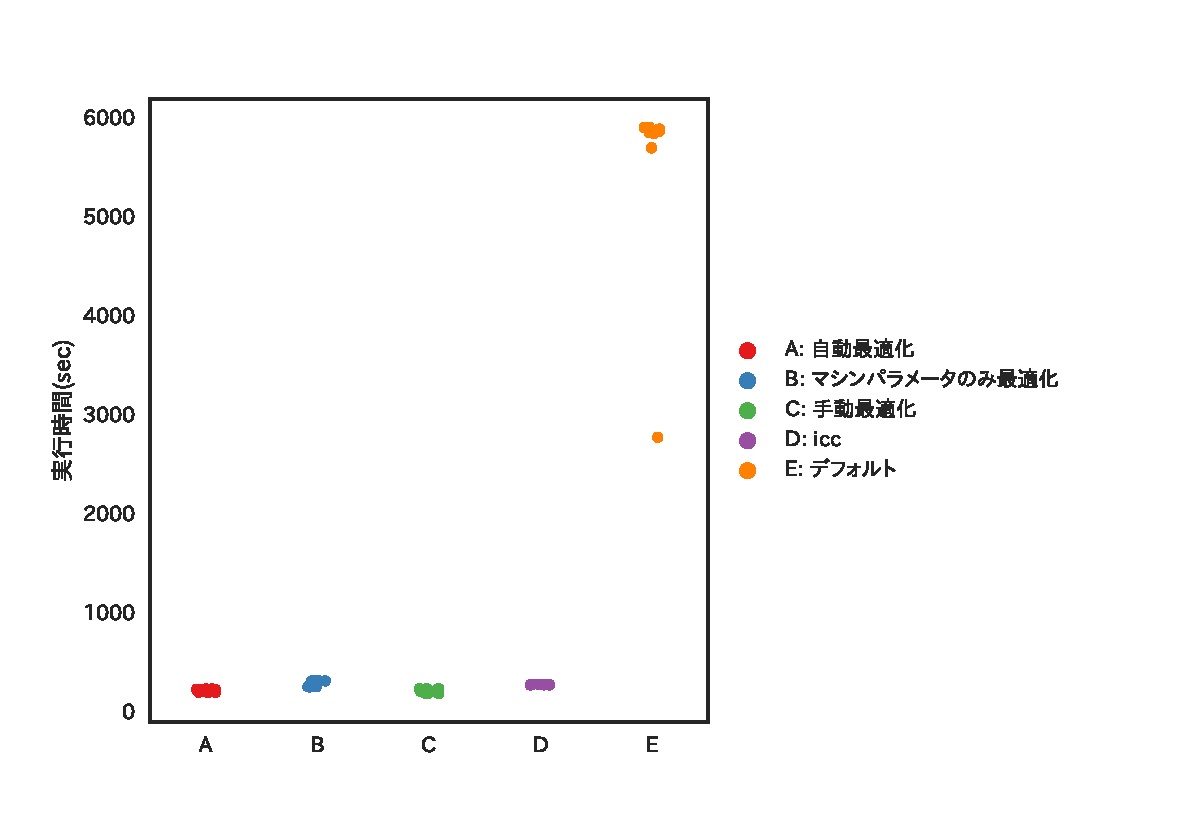
\includegraphics[width=14cm]{./images/cluster-compare.pdf}
    \caption{クラスタ 自動最適化評価}
    \label{fig:cluster-compare}
  \end{center}
\end{figure}~\\
次にデフォルトを除いた他の4つの条件のみを図\ref{fig:cluster-compare-2}に示す.\\
\begin{figure}[htb]
% h:here, t:top, b:bottom, p:page
 \begin{center}
    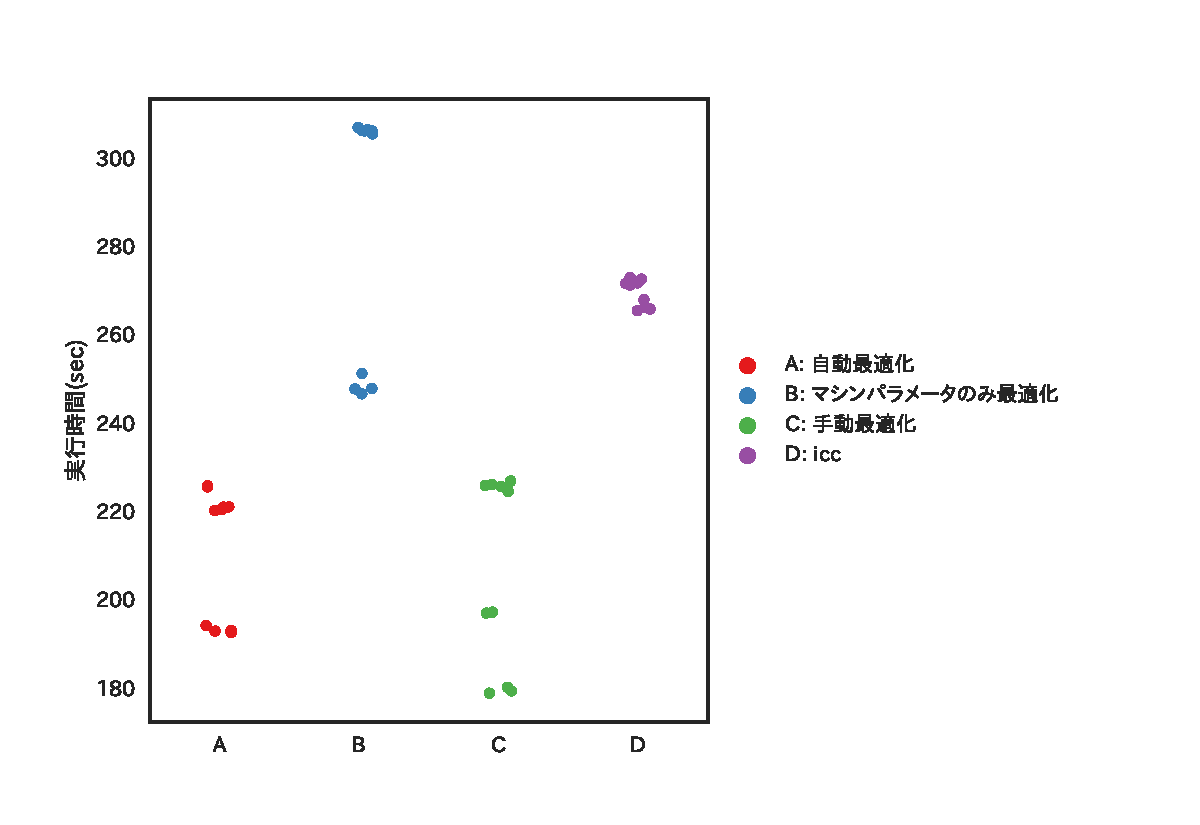
\includegraphics[width=14cm]{./images/cluster-compare-2.pdf}
    \caption{クラスタ 自動最適化評価 (デフォルト以外)}
    \label{fig:cluster-compare-2}
  \end{center}
\end{figure}~\\
この図から, 自動最適化を行ったものは手動での最適化と比べ多少劣るものの,
マシンパラメータのみの最適化を行ったものや最適化に非常に優れたコンパイラであるiccを用いたもの比較しても
十分に高速化されているといえる.\\
\subsubsection{京}~\\
同様にして京においての比較結果を図\ref{fig:k-compare}に示す.
クラスタの結果と比べ特徴的なのは, 個々のシミュレーションの実行時間にばらつきがないことで
これは京においてログインノードと計算用のノードが分離されているため, シミュレーションが別プロセスの影響を受けにくいからであると考えられる.\\
\begin{figure}[htb]
% h:here, t:top, b:bottom, p:page
 \begin{center}
    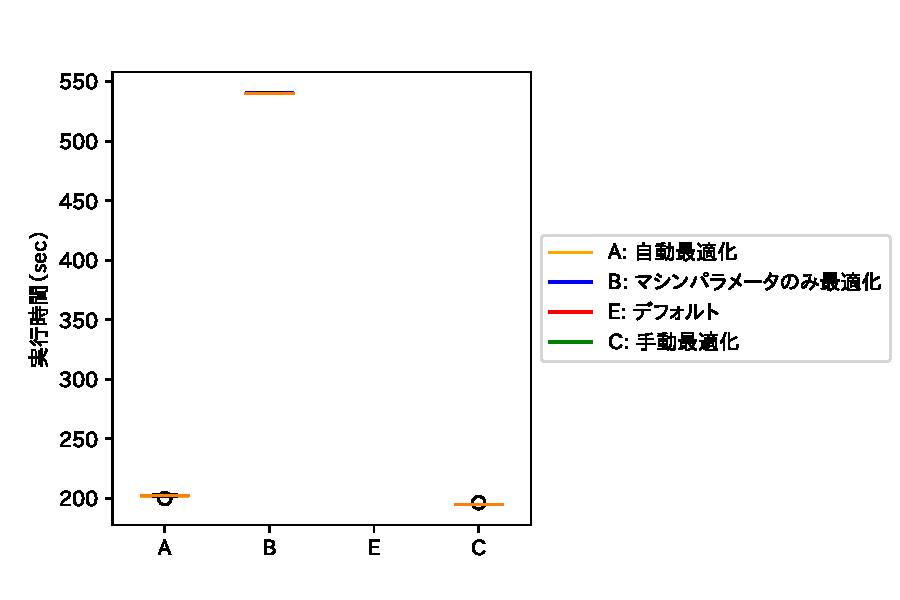
\includegraphics[width=14cm]{./images/k-compare.pdf}
    \caption{京 自動最適化評価}
    \label{fig:k-compare}
  \end{center}
\end{figure}~\\

最後に自動最適化と手動最適化のみを比較したものを図\ref{fig:k-compare-2}に示す.\\
先行研究で行われた手動最適化は, この京環境に対して行われていたためクラスタでの実行よりも顕著に差が現れている.
しかしながらその差は全体の1割にもみたないため, 自動最適化によるシミュレーションの高速化は京環境においても十分な効果を発揮したといえる.\\
さらに, 最適化アルゴリズムの追加やベンチマークなどの改良を行うことでこの差を埋めることも可能であると考える.\\
\begin{figure}[htb]
% h:here, t:top, b:bottom, p:page
 \begin{center}
    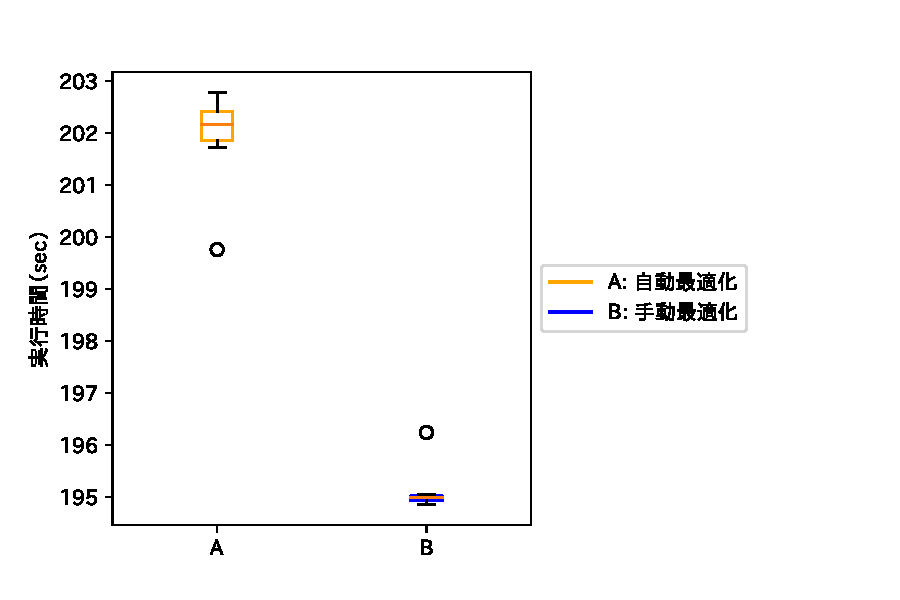
\includegraphics[width=14cm]{./images/k-compare-2.pdf}
    \caption{京 自動最適化評価(自動 vs 手動)}
    \label{fig:k-compare-2}
  \end{center}
\end{figure}~\\
